%!TEX root = kPtx_paper.tex
\section*{Results}

\begin{figure}
	\centering
	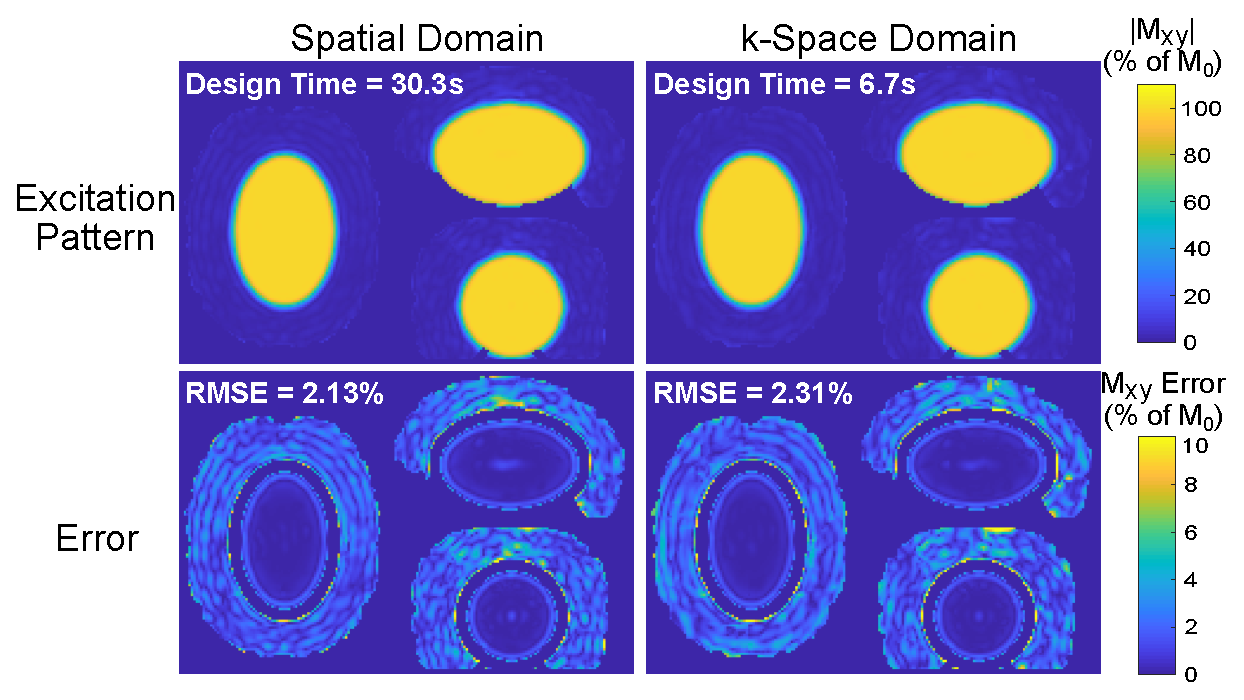
\includegraphics[width=\textwidth]{ErrorMap}
	\caption{\textcolor{red}{WAG: I think this is the figure that your example in Github should replicate.}
	Normalized excitation patterns (top row) and error maps (bottom row) in central axial, sagittal and coronal slices 
	for k-space domain (left) and spatial domain designs (right).}
	\label{fig:ErrorMap}
\end{figure}
Figure \ref{fig:ErrorMap} shows simulated excitation patterns and error maps for the reference spatial and k-space domain designs. 
Both designs were performed with 16 parallel threads and the 64$\times$64$\times$48 grid size (3 mm isotropic resolution), 
and the excitation patterns were evaluated against the target pattern on a 128$\times$128$\times$96 grid size (1.5 mm iso-resolution). 
The k-space domain design used patch and inclusion widths of 4.
The calculated root-mean-squared errors (RMSEs) were 2.42\% (spatial domain) and 2.68\% (k-space domain), 
respectively. 
For both design methods, most of the errors appeared at the edges of the transition band, 
and errors elsewhere were lower than 5\% of the target flip angle. 
This indicates uniform inner volume excitation while maintaining the outer volume intact. 
The parallelized k-space domain design required 2.9 seconds computation versus 31.8 seconds for the spatial domain method, a 91\% decrease.

\begin{figure}
	\centering
	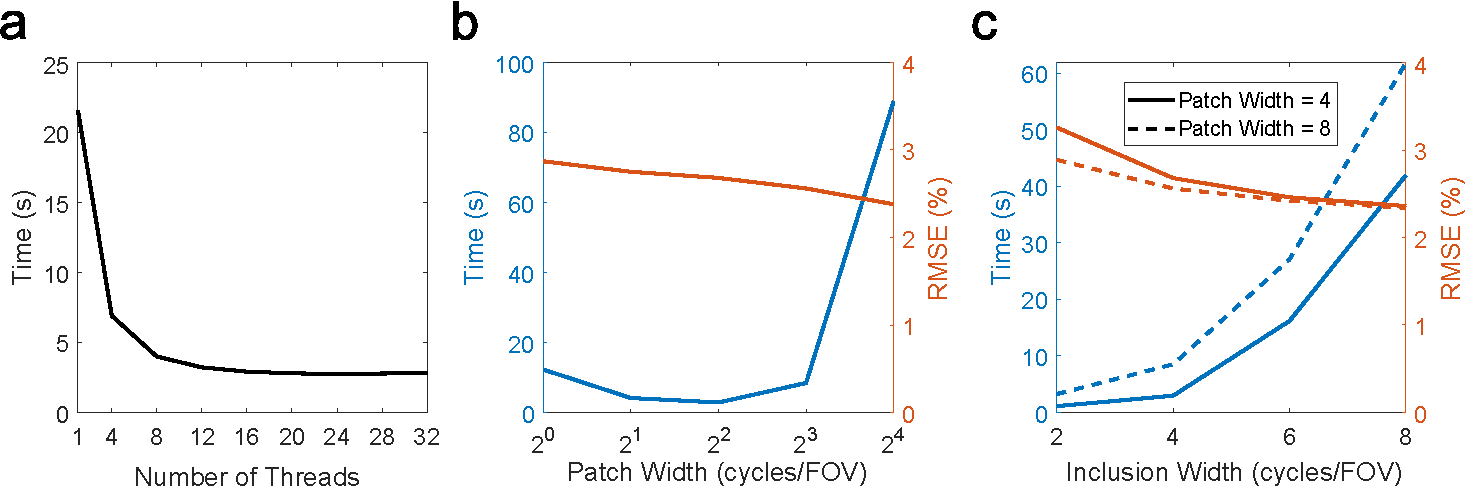
\includegraphics[width=\textwidth]{ComputationTime}
	\caption{(a) k-Space computation time versus number of parallel threads, for patch and inclusion widths of 4 cycles/FOV. 
	(b) Computation time (blue axis) and RMSE (red axis) versus patch width, for an inclusion width of 4 cycles/FOV and 16 threads. 
	(c) Computation time (blue axis) and RMSE (red axis) versus inclusion width, for patch widths of 4 and 8 cycles/FOV, and 16 threads.}
	\label{fig:ComputationTime}
\end{figure}
\subsection*{k-Space Algorithm Parameters}
Figure \ref{fig:ComputationTime}a plots mean computation time versus number of parallel threads,
holding the patch and inclusion widths fixed at 4 cycles/FOV. 
The computation time decreased rapidly with increasing thread number up to 12 threads, 
and then plateaued, likely due to the overhead involved in initiating threads after that point.
Based on this result, the number of threads was held fixed at 16 for subsequent designs when off-resonance was not compensated.

\par Figure \ref{fig:ComputationTime}b plots mean computation time and RMSE with different patch widths. 
The computation time decreased up to a patch width of 4 cycles/FOV (corresponding to $4^3 = 64$ simultaneously solved columns of $\bm{W}$) 
and then increased sharply for larger patch widths. 
RMSE decreased slowly as the patch width increased since the number of excitation trajectory points included in the calculation of weights for each 
target point increases on average (and especially for target locations in the middle of each patch) as the patch width increases, 
even when the inclusion width stays fixed.
Based on this result, a patch width of 4 cycles/FOV was used for subsequent designs.

\par Figure \ref{fig:ComputationTime}c plots mean computation time and RMSE with different inclusion widths. 
The solid lines and dashed lines were obtained with patch widths of 4 and 8 cycles/FOV, respectively. 
Computation time increased and error decreased with increasing inclusion width,
since more excitation trajectory points were included in each target location's calculation for increasing inclusion width,
corresponding to an increased $\bm{S}^H\bm{S}$ matrix size. 
The RMSE was only slightly lower for a patch width of 8 versus 4 cycles/FOV, 
but the computation time was much higher for 8 cycles/FOV, across all inclusion widths. 
The knees in the curves occurred approximately at an inclusion width of 4 cycles/FOV,
so this value was used in subsequent designs. 

\par Table \ref{fig:wsize} lists the size of the final matrix $\bm{W}$ in gigabytes,
versus inclusion width.
As inclusion width increases, more excitation trajectory points are used in the solution of the weights for each target location,
until the entire trajectory is used for each location (Inclusion width = $\infty$ in the table),
corresponding to a full solution. 
With the inclusion width of 4 cycles/FOV used here, 
the matrix size was 98\% smaller than that of a full solution.  

\begin{figure}
\centering
\begin{tabular}{c | c}
Inclusion Width & $\bm{W}$ Matrix Size (GB) \\
\hline
$\infty$ & 24.4 \\
8 & 2.73 \\
6 & 1.37 \\
4 & 0.53 \\
2 & 0.14
\end{tabular}
\caption{$\bm{W}$ matrix sizes in gigabytes (GB) versus inclusion width in cycles/FOV. 
An inclusion width of $\infty$ corresponds to a full matrix solution.}
\label{fig:wsize}
\end{figure}

\begin{figure}
	\centering
	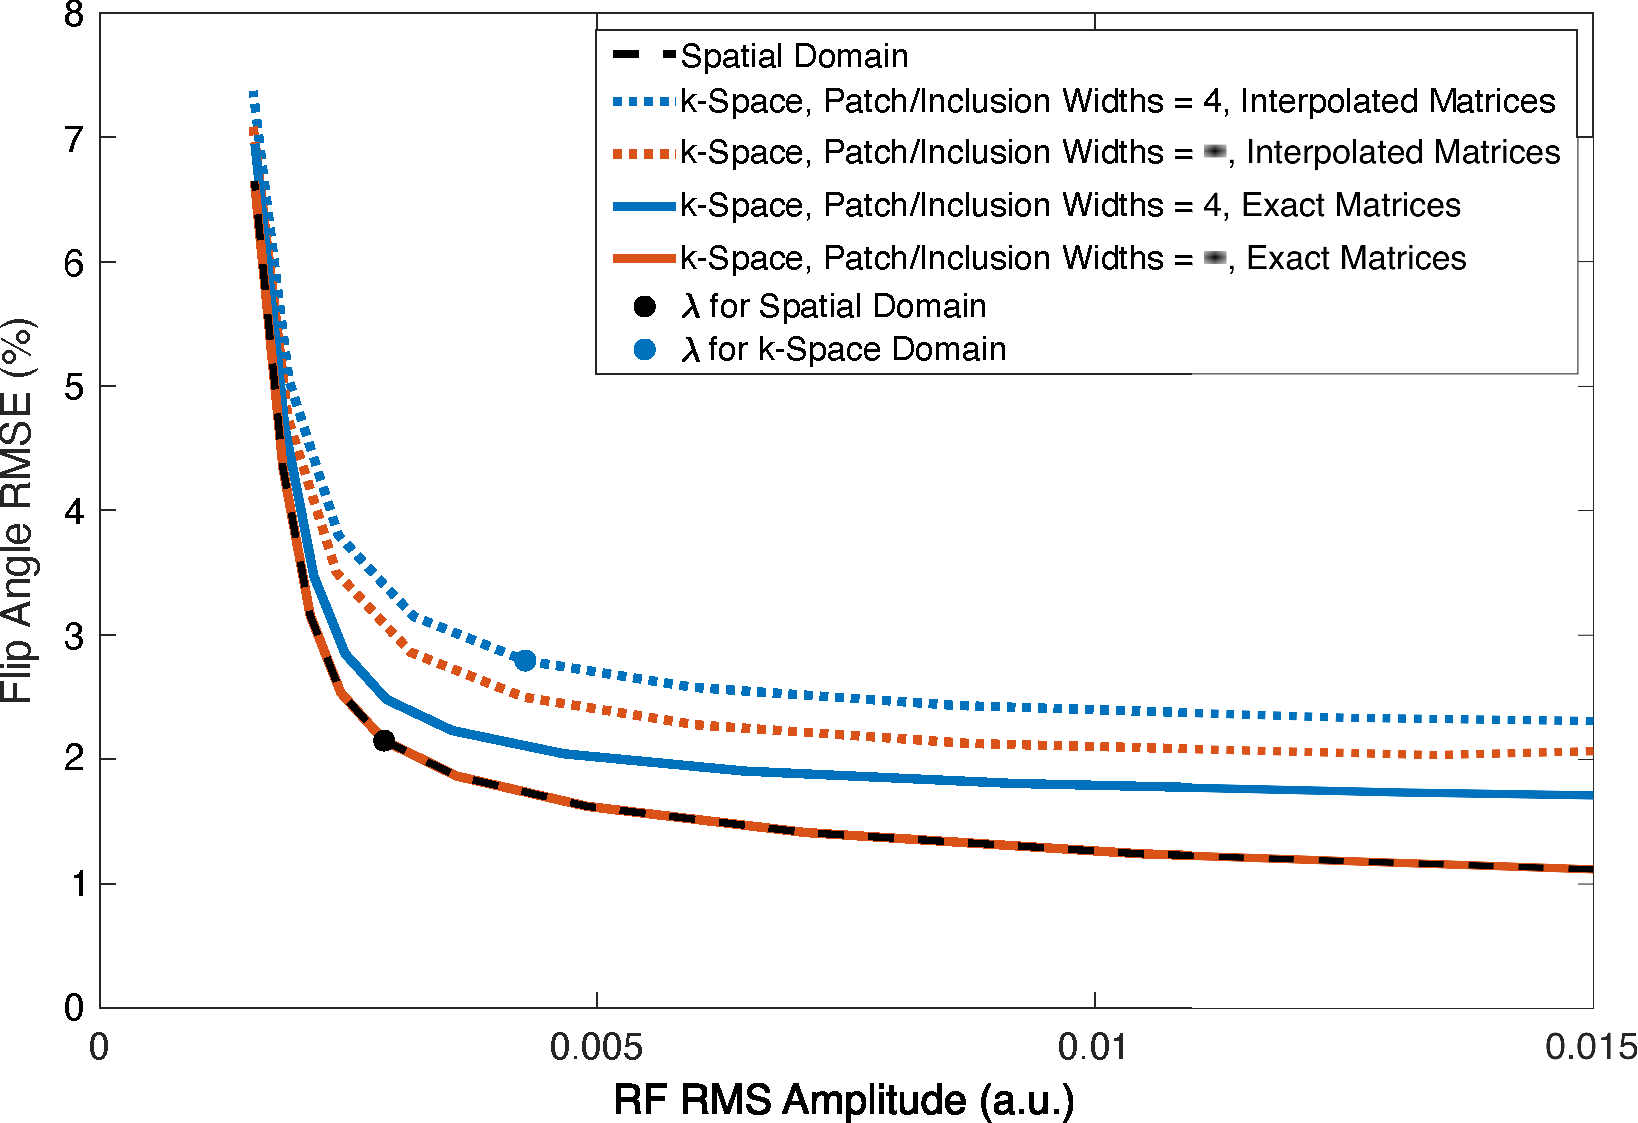
\includegraphics[width=\textwidth]{L_curve}
	\caption{L-curves for spatial domain and k-space domain pulse designs, 
	repeated across five orders of magnitude of the methods' Tikhonov regularization parameters.
	The k-space domain designs were repeated using patch and inclusion widths of four versus solving for the entire domain at once (`Patch / Inclusion Width = 4' versus `Full Patch'),
	and using $B_1^+$ map product interpolation versus phase modulation to each trajectory location (`Interpolated $\bm{S}^H\bm{S}$ Matrices' versus
	`Exact $\bm{S}^H\bm{S}$ Matrices').}
	\label{fig:LCurves}
\end{figure}

\subsection*{L-Curves}
Figure \ref{fig:LCurves} plots flip angle RMSE versus RF RMS amplitude for the spatial domain method
and different configurations of the k-space domain method.
The spatial domain method achieves the best overall tradeoff between error and RMS amplitude (dashed black curve),
which is matched by the k-space domain method when all target locations are solved simultaneously with
all excitation trajectory points included and exact $\bm{S}^H\bm{S}$ matrix construction (orange curve). 
When the inclusion and patch widths are limited to 4 cycles/FOV but the $\bm{S}^H\bm{S}$ 
matrices are still constructed exactly, there is an increase in error and RMS amplitude (solid blue curve). 
However, a larger penalty is incurred by interpolating the entries of the $\bm{S}^H\bm{S}$ matrices (dashed orange curve)
than by limiting the inclusion and patch widths.
Combining interpolation of the $\bm{S}^H\bm{S}$ matrix entries and patch and inclusion widths of 4 cycles/FOV yield 
the dashed blue curve, which has a higher error and RF amplitude than when interpolation or small patch and inclusion widths are
used alone.
Overall, these results and the results in Figure \ref{fig:ComputationTime} and Table \ref{fig:wsize}
show that the k-space domain method allows a tradeoff between computation time and memory usage versus
excitation error and RMS RF amplitude.
The dots on the spatial domain and k-space domain curves indicate the knees of of the curves corresponding to
the $\lambda$ values used for the designs in Figures \ref{fig:ErrorMap}, \ref{fig:ComputationTime}, \ref{fig:kspace_PTX_Acceleration}, and \ref{fig:kspace_PTX_B0}.
Note that the RMSE's in Figure \ref{fig:LCurves} are slightly lower for the spatial domain designs
and slightly higher for the k-space domain designs compared to other figures,
because the flip angle errors in Figure \ref{fig:LCurves} were calculated using 
spatial domain non-uniform fast Fourier transforms instead of Bloch equation simulations, 
to provide a more direct measure of the design error. 

\begin{figure}
	\centering
	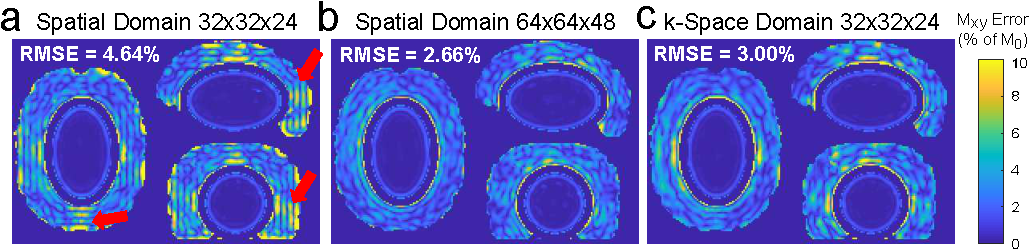
\includegraphics[width=\textwidth]{GibbsRinging}
	\caption{Normalized error maps and RMSE for \textbf{(a)} spatial domain design and \textbf{(c)} k-space domain design with 6 mm iso-resolution, 32$\times$32$\times$24 design grid. Red arrows indicate the Gibbs ringing in low-resolution spatial domain design. \textbf{(b)} Normalized error map for spatial domain design with 3 mm iso-resolution, 64$\times$64$\times$48 design grid.}
	\label{fig:GibbsRing}
\end{figure}

\subsection*{Gibbs Ringing}
Figure \ref{fig:GibbsRing}a shows slices of the excitation error pattern produced by pulses designed by the spatial domain method
on a 32$\times$32$\times$24 grid, which were Bloch-simulated on the original 128$\times$128$\times$96 grid. 
There is significant Gibbs ringing in the pattern (indicated by the red arrows),
and the pulses incur a higher RMSE (4.64\%) than pulses designed using either the spatial domain method with a finer 64$\times$64$\times$48 grid
(2.66\%; Figure \ref{fig:GibbsRing}b) or the k-space domain method with a 32$\times$32$\times$24 grid (3.00\%; Figure \ref{fig:GibbsRing}c). 
Gibbs ringing is not apparent in either the 64$\times$64$\times$48 spatial domain error pattern or the 32$\times$32$\times$24 k-space domain error pattern. 
The RMS RF amplitudes of the low resolution designs were both 0.05. 
Note that the error of the 64$\times$64$\times$48 spatial domain design is slightly higher than designs presented in other figures
due to the lower-resolution excitation trajectory. 
From a spatial domain point of view, 
the Gibbs ringing in the low-resolution spatial domain design was caused by the design's inability to observe and limit the ringing in the low-resolution design grid. 
From a k-space domain point of view, the Gibbs ringing in 
Figure \ref{fig:GibbsRing}a was due to implicit circulant end conditions at the edges of excitation k-space in the low-resolution
spatial domain design,
which led RF samples at one edge of k-space to wrap-around and affect target locations at the opposite edge of k-space. 
This effect is mitigated using a high-resolution spatial domain design grid, as illustrated in Figure \ref{fig:GibbsRing}b. 
However, even for a low-resolution k-space domain design there is no wrap-around effect in excitation k-space 
because the trajectory points that are incorporated in the weights solution for each patch of target locations are explicitly specified to be those in the immediate vicinity of 
the target points, without circulant end conditions. 
%Particularly, for the instance problems whose patches are at the edges of the k-space FOV, the excitation trajectory points at the other ends of the k-space FOV will not be incorporated into the design.    

%Due to implicit circulant end conditions in k-space for the spatial domain design, t

\begin{figure}
	\centering
	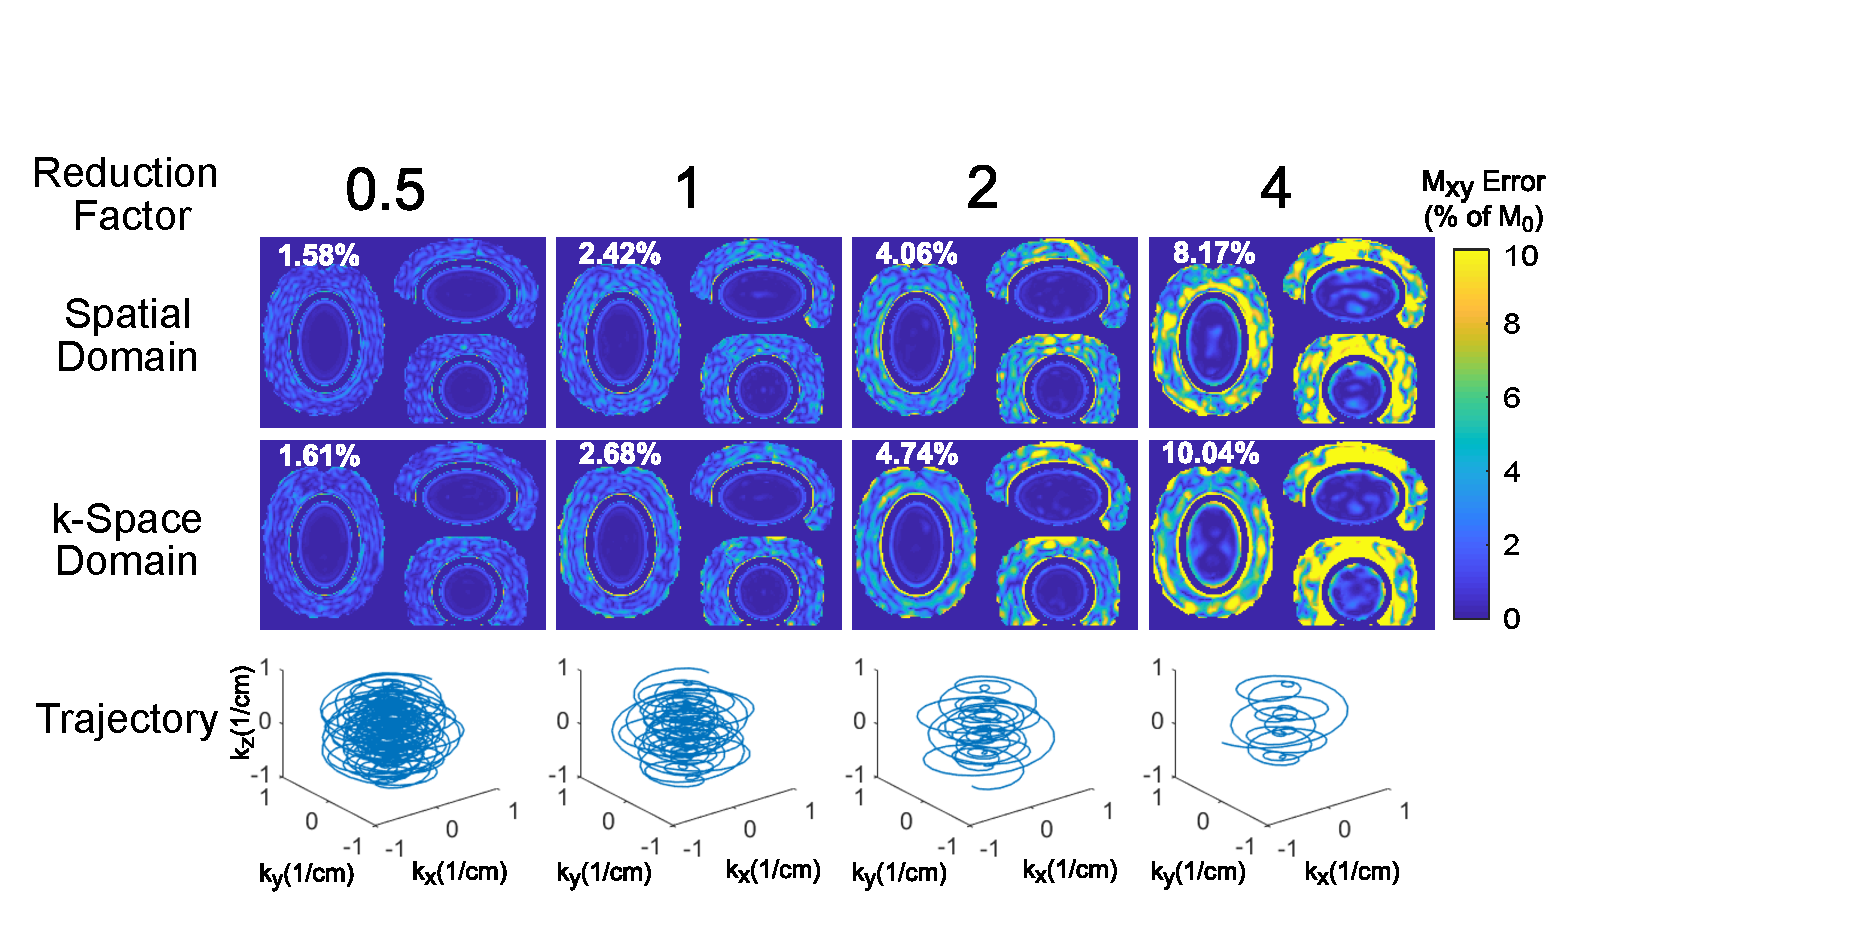
\includegraphics[width=\textwidth]{ReductionFactor}
	\caption{Normalized error maps and RMSEs for spatial domain design (first row) and k-space domain design (second row), 
	using excitation k-space trajectories with different reduction factors (third row).
	The reduction factors are referenced to the 10 ms trajectory in Figure \ref{fig:Target} (second column).}
	\label{fig:kspace_PTX_Acceleration}
\end{figure}

\subsection*{Excitation k-Space Undersampling}
Figure \ref{fig:kspace_PTX_Acceleration} compares excitation error patterns produced by spatial domain-designed pulses (top row)
and k-space domain-designed pulses (middle row),
for different trajectory reduction factors which resulted in the SPINS trajectories plotted in the third row. 
For each design the k-space domain-designed pulses had higher error, 
but error increased smoothly with increasing reduction factor, as it did for the spatial domain designs. 


\begin{figure}
	\centering
	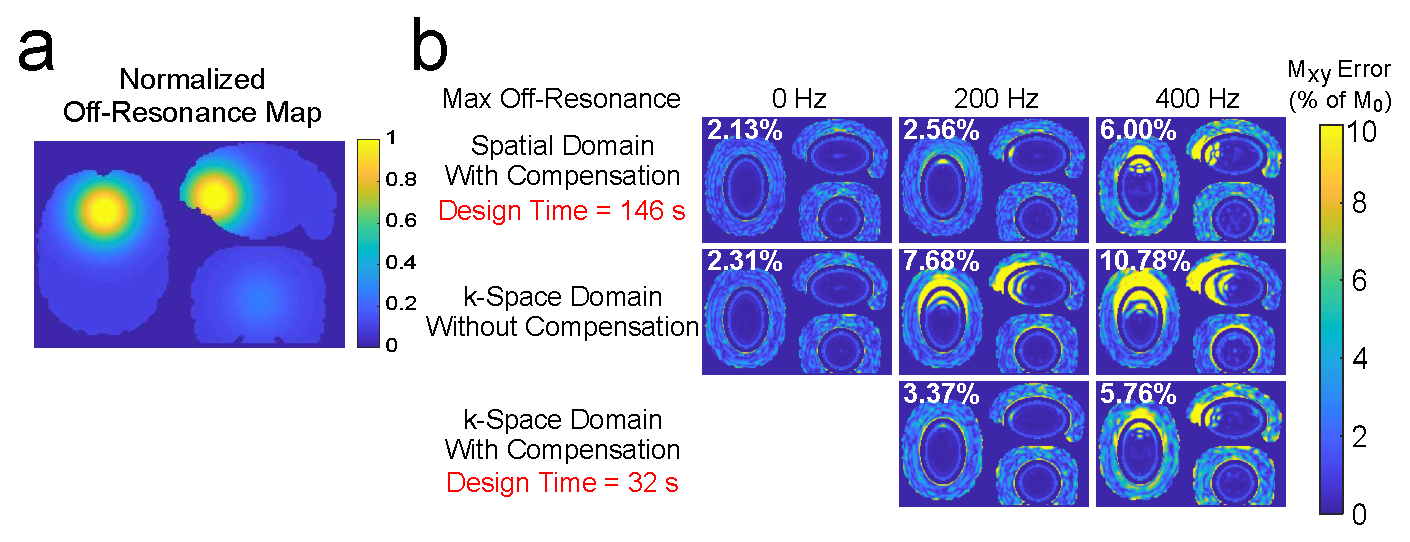
\includegraphics[width=\textwidth]{OffResonance}
	\caption{
	(a) Normalized off-resonance map containing a Gaussian distortion centered above the frontal sinus, 
	to mimic air-tissue susceptibility difference-induced $B_0$ inhomogeneity.
	(b) Normalized excitation maps and RMSEs for spatial domain design with off-resonance correction (first row), 
	and k-space domain design without and with off-resonance correction (second and third rows).}
	\label{fig:kspace_PTX_B0}
\end{figure}

\subsection*{Off-Resonance}
Figure \ref{fig:kspace_PTX_B0}a shows the off-resonance maps containing a Gaussian distortion which was centered above the frontal sinus,
and scaled to peak amplitudes of 0, 200, and 400 Hz for the pulse designs and Bloch simulations. 
Figure \ref{fig:kspace_PTX_B0}b shows excitation error patterns and RMSEs for spatial domain designs with off-resonance compensation,
and k-space domain designs without and with off-resonance compensation. 
Without off-resonance compensation, 
the k-space domain-designed pulses produced large ($>$ 10\% of $M_0$) excitation errors both inside and outside the target ellipse. 
When the off-resonance map was incorporated in the spatial domain and k-space domain designs, 
the distortion was nearly fully corrected when it had a peak amplitude of 200 Hz. 
When the map was scaled to a peak of 400 Hz, some large errors remained, with the k-space domain-designed pulses achieving slightly lower RMSE. 
%It was also able to provide excitation pattern comparable to spatial domain design with 400 Hz maximum off-resonance. The k-space domain design has a weaker performance with higher off-resonance due to the fact that the time segmentation approximation in Ref \cite{fessler2005toeplitz} was meant to approximate forward models from RF to excitation patterns and does not serve as an accurate approximation to the backward model as we need in the k-space domain design.